% =============================================================
%  Question2.tex —— 问题二：考虑时间窗惩罚的单车辆路径规划
%  数据来源：results/基础模型/q2_pure_python.json
%             results/改进模型/q2_pure_python_v2.json
%             results/基础模型/qubo_v1_q2_kaiwu_sdk.json
%             results/真机结果/q2/  R-Q2-006
%             paper/章节/00_实验日志_问题二.md
%  编译方式：xelatex Question2.tex
% =============================================================
\documentclass[UTF8,12pt,a4paper]{ctexart}

\usepackage{amsmath}
\usepackage{amssymb}
\usepackage{geometry}
\geometry{margin=2.5cm}
\usepackage{booktabs}
\usepackage{float}
\usepackage{caption}
\usepackage{graphicx}
\graphicspath{{../../../figures/}}

% 与全文章节编号对齐：本节在主稿中为第 7 节
\setcounter{section}{6}

\begin{document}

% =============================================================
\section{问题二：考虑时间窗惩罚的单车辆路径规划}
\label{sec:q2}
% =============================================================

% -------------------------------------------------------------
\subsection{问题二分析}
% -------------------------------------------------------------

问题二在问题一的单车辆 TSP 基础上引入\textbf{软时间窗惩罚}：每个客户 $i$ 给定服务窗
$[a_i,b_i]$，车辆仍允许早到或迟到，但按二次罚函数计入目标。题目同时规定
\textbf{无空闲等待}，即车辆若早于时间窗下界到达，仍立即开始服务，并按早到量产生惩罚；
迟到同理。罚系数取 $M_1=10,\ M_2=20$，分别对应早到与迟到。本问的求解目标因此从问题一
的"最短运输时间"扩展为"运输时间 $+$ 软时间窗惩罚"的综合目标，需要在二者之间权衡。
本问在全文中的作用是：（i）在 $n=15$ 小规模上验证软时间窗约束下的 QUBO 编码方案；
（ii）通过对比"QUBO 内线性化"与"解码后回评"两种处理方式，给出问题三大规模分解所采用
的编码取舍依据；（iii）保持 Python / Kaiwu SDK / CIM 真机的三层一致验证链路。

% -------------------------------------------------------------
\subsection{服务开始时刻递推与时间窗惩罚}
\label{subsec:q2-time}
% -------------------------------------------------------------

记访问序列为 $\pi=(\pi_0,\pi_1,\dots,\pi_n,\pi_{n+1})$，其中 $\pi_0=\pi_{n+1}=0$ 为
配送中心，$\{\pi_1,\dots,\pi_n\}$ 为 $\{1,\dots,n\}$ 的一个排列；$T_{ij}$ 为节点 $i,j$
之间的旅行时间，$s_i$ 为客户 $i$ 的服务时间。在"无空闲等待"假设下，访问序号 $k$ 处的
客户开始服务时刻 $t_{\pi_k}$ 按下式递推：
\begin{align}
t_{\pi_1} &= T_{0,\pi_1},
   \label{eq:q2-t-first}\\[2pt]
t_{\pi_k} &= t_{\pi_{k-1}} + s_{\pi_{k-1}} + T_{\pi_{k-1},\pi_k},\qquad k=2,\dots,n,
   \label{eq:q2-t-rec}
\end{align}
即使 $t_{\pi_k} < a_{\pi_k}$ 也立即开始服务而不等待。回到配送中心的总运输时间单独由
\begin{equation}
\label{eq:q2-travel}
\mathrm{travel}(\pi) = T_{0,\pi_1} + \sum_{k=1}^{n-1} T_{\pi_k,\pi_{k+1}} + T_{\pi_n,0}
\end{equation}
计算，其中 $\mathrm{travel}$ 仅累加边权而不含服务时间。客户 $i$ 的二次时间窗罚函数为
\begin{equation}
\label{eq:q2-penalty}
P_i(t_i) \;=\; M_1\bigl[a_i - t_i\bigr]_{+}^{2} + M_2\bigl[t_i - b_i\bigr]_{+}^{2},\qquad
M_1 = 10,\ M_2 = 20,
\end{equation}
其中 $[x]_{+}=\max(x,0)$；$P_i(t_i)>0$ 当且仅当 $t_i \notin [a_i,b_i]$。综合业务目标为
\begin{equation}
\label{eq:q2-J}
J(\pi) \;=\; \mathrm{travel}(\pi) \;+\; \sum_{i=1}^{n} P_i(t_i),
\end{equation}
其中 $\mathrm{travel}$ 是车辆在弧上累计的运输时间；$P_i(t_i)$ 是客户 $i$ 的时间窗惩罚；
$J$ 是问题二真正要最小化的业务目标，与下文 §\ref{subsec:q2-enc} 中 QUBO 形式的能量
$H$ 相区分——\textbf{$H$ 仅承担路径排序的二次约束与运输时间项，时间窗惩罚通过解码后
按式~\eqref{eq:q2-penalty} 回评，再代入式~\eqref{eq:q2-J} 计算 $J$}。

% -------------------------------------------------------------
\subsection{QUBO 编码方案比较与主方案选择}
\label{subsec:q2-enc}
% -------------------------------------------------------------

问题二难点不在路径本身的二次组合结构，而在时间窗罚 $[a_i-t_i]_+^{2}$、$[t_i-b_i]_+^{2}$
是依赖前缀路径累计时间的\textbf{多次型动态量}。若直接展开为 QUBO 二次形，需要为
"位置 $p$ 的累计到达时刻"额外引入大量时间槽辅助比特，显著增加变量规模并破坏稀疏性。
本文比较以下四种编码方案后选定主方案，结果汇总于表~\ref{tab:q2-enc}：

\begin{table}[H]
  \centering
  \caption{问题二 QUBO 编码方案比较}
  \label{tab:q2-enc}
  \footnotesize
  \begin{tabular}{lcccccl}
    \toprule
    方案 & 比特数 & 二次性 & 原始可行率 & 解码后 $J$ & 取舍 \\
    \midrule
    A 显式时刻槽位 & $\sim 900$ & 满足 & 未实施 & 未实施 & 比特规模过大 \\
    B 位置 binary 编码 & $\sim 60$ & 不满足 & 未实施 & 未实施 & 破坏 QUBO 二次性 \\
    \textbf{C one-hot $+$ 解码后回评（主方案）} & \textbf{225} & 满足 & 0.6\% & \textbf{84121} & 主方案 \\
    D one-hot $+$ TW 线性化（消融对照） & 225 & 满足 & 0\% & 无可行解 & 仅作消融对照 \\
    \bottomrule
  \end{tabular}
\end{table}

\textbf{方案 C（主方案）：one-hot 编码 $+$ 解码后回评。} 沿用问题一的位置 one-hot 变量
$x_{i,p}\in\{0,1\}$（$i,p=1,\dots,n$，共 $n^{2}=225$ 比特），将式~\eqref{eq:q2-qubo} 的
QUBO 写为
\begin{equation}
\label{eq:q2-qubo}
H(\mathbf{x}) \;=\; \underbrace{A\sum_{p=1}^{n}\!\Big(\!\sum_{i} x_{i,p}-1\Big)^{2}
+ A\sum_{i=1}^{n}\!\Big(\!\sum_{p} x_{i,p}-1\Big)^{2}}_{H_{\rm onehot}}
\;+\; \underbrace{H_{\rm travel}(\mathbf{x})}_{\text{形如式}~\eqref{eq:q2-travel}\text{的 QUBO 形式}},
\end{equation}
其中 $H_{\rm onehot}$ 为 one-hot 二次罚项（$A=200$，沿用问题一），$H_{\rm travel}$ 即
式~\eqref{eq:q2-travel} 的 QUBO 化形式（与 §6.3 的 $H_{\rm travel}$ 同构）。\textbf{时间
窗惩罚 $\sum_i P_i(t_i)$ 不进入 QUBO}，而是在 spin 解码为合法路径 $\pi$ 后，由统一
\texttt{evaluate} 函数按式~\eqref{eq:q2-t-rec}--\eqref{eq:q2-J} 回评，并作为业务目标 $J$
参与候选解筛选与最终结果评价。该方案保持 225 比特、保留二次性、避免动态时间窗递推被
强行展开，是本文的主方案。

\textbf{方案 D（消融对照）：QUBO 内线性化时间窗。} 假设位置 $p$ 处的到达时刻可由"前 $p-1$
个位置上的客户期望服务时间"近似为线性表达 $\hat\tau_p$，将 $\hat P_i\approx
M_2(\hat\tau_p-b_i)^{2}$ 直接以 $x_{i,p}$ 的对角项加入 QUBO。实测中，$\hat P_i$ 的对角线
峰值约为 $1.2\times 10^{5}$，相对 one-hot 罚 $A=200$ 形成 $\sim$596 倍的尺度差，导致 SA
会优先把所有 $x_{i,p}\!=\!0$ 来消去对角巨值，one-hot 约束 $\sum_p x_{i,p}=1$ 全部失效，
原始可行率 0\%。方案 D 因此\textbf{仅作为消融对照存在，不是最终模型}。该现象说明：动态
时间窗惩罚不适合直接粗暴塞入 QUBO 对角项，更适合在解码阶段通过统一评价函数处理。本文
据此采用比特预算与约束尺度原则——将路径二次结构留给 QUBO，将动态/多次型约束留给解码
后的回评。

% -------------------------------------------------------------
\subsection{三层求解算法设计}
\label{subsec:q2-algo}
% -------------------------------------------------------------

针对方案 C 的 225 比特 QUBO 与综合目标 $J$ 的高度非凸特性（$\mathrm{travel}$ 与
$\sum_i P_i$ 通常呈\textbf{反向}：缩短 $\mathrm{travel}$ 可能加剧晚到罚），本文设计四层
异构求解流水线，全部以同一 \texttt{evaluate} 函数评价 $J$ 以保证可比性：
\begin{enumerate}
  \item[(i)] \textbf{纯 Python v1（多起点 $+$ SA）}：13 个 warm-start（8 个随机 $+$
    Nearest Neighbor $+$ 时间窗紧迫度排序等），配合 2-opt / Or-opt / swap 三件套局部
    搜索与 SA（$T_0=80,\alpha=0.995$）。
  \item[(ii)] \textbf{纯 Python v2（多起点 $+$ LNS $+$ 多 seed SA）}：27 个 warm-start，
    150 轮 LNS（ruin-and-recreate $+$ regret-2 重插），3 个 SA 种子，配合 3-opt 重型精修。
  \item[(iii)] \textbf{Kaiwu SDK SA}：对式~\eqref{eq:q2-qubo} 转化的 Ising 矩阵调用
    \texttt{SimulatedAnnealingOptimizer}（5 seeds $\times$ 200 chains $=1\,000$ 候选解，
    $T_0=500,\alpha=0.995$，NN warm-start）；对所有可行候选统一 polish 取 $J$ 最优。
  \item[(iv)] \textbf{CIM 真机求解}：将 $226\times 226$、8-bit 精度的 Ising 矩阵上传至
    玻色 CPQC-550，任务编号 R-Q2-006，获取 10 个独立 spin 样本后 polish 精修。
\end{enumerate}
其中需特别说明的关键技巧是：\textbf{QUBO 能量最优 $\ne J$ 最优}，因此在 SDK / CIM 阶段
不能仅取能量最低的样本作为最终解，而需对能量序前若干可行候选共同 polish 后按 $J$ 取最优。

% -------------------------------------------------------------
\subsection{求解结果与调度解释}
\label{subsec:q2-result}
% -------------------------------------------------------------

四类求解器在 $n=15,\ A=200,\ M_1=10,\ M_2=20$ 下的对比结果如表~\ref{tab:q2-cmp}。

\begin{table}[H]
  \centering
  \caption{问题二三层求解器对比（均使用同一 \texttt{evaluate} 函数评价 $J$）}
  \label{tab:q2-cmp}
  \footnotesize
  \begin{tabular}{lccccccc}
    \toprule
    求解方式 & 候选数 & 原始可行率 & travel & penalty & $J$ & 耗时/s & 说明 \\
    \midrule
    Python v1（多起点 $+$ SA）       & 13    & 100\%  & 31 & 84\,090 & \textbf{84\,121} & 21    & 经典基线 \\
    Python v2（多起点 $+$ LNS $+$ 多 seed SA） & 27    & 100\%  & 31 & 84\,090 & \textbf{84\,121} & 56    & 增强基线 \\
    Kaiwu SDK SA                          & 1\,000 & 0.6\%  & 31 & 84\,090 & \textbf{84\,121} & 3.84  & QUBO 验证 \\
    CIM 真机 R-Q2-006                     & 10    & 10\%   & 31 & 84\,090 & \textbf{84\,121} & 122.3 & 真机验证 \\
    \bottomrule
  \end{tabular}
  \begin{flushleft}\footnotesize
  注：$\mathrm{travel}$、$\mathrm{penalty}$、$J$ 均由原始未量化的 $T_{ij}$ 与
  式~\eqref{eq:q2-t-rec}--\eqref{eq:q2-J} 计算，与 QUBO 能量 $H$ 区分。CIM 耗时
  122.3 s 为平台端到端时间（排队 $+$ 上传 $+$ 采样），待核对。
  \end{flushleft}
\end{table}

由表~\ref{tab:q2-cmp} 可知，最优访问路径序列为
\begin{equation}
\label{eq:q2-route}
0\to 2\to 13\to 6\to 5\to 8\to 7\to 11\to 10\to 1\to 9\to 3\to 12\to 4\to 15\to 14\to 0,
\end{equation}
对应路径图见图~\ref{fig:q2-route}。Python v1/v2、Kaiwu SDK 与 CIM 真机四类异构求解器
均得到相同的最优可行解 $J=84\,121$（$\mathrm{travel}=31$，$\mathrm{penalty}=84\,090$）。
该一致性是结果可信度的重要证据：跨算法（多起点启发式 / LNS / SA / 量子退火）$\times$
跨硬件（CPU / 玻色 CPQC-550）$\times$ 跨平台（本地 Python / Kaiwu SDK / 云端真机）三条
独立链路落在同一最优解上，增强了结果稳定性证据；在已测试算法邻域内未发现更优解。

\begin{figure}[H]
  \centering
  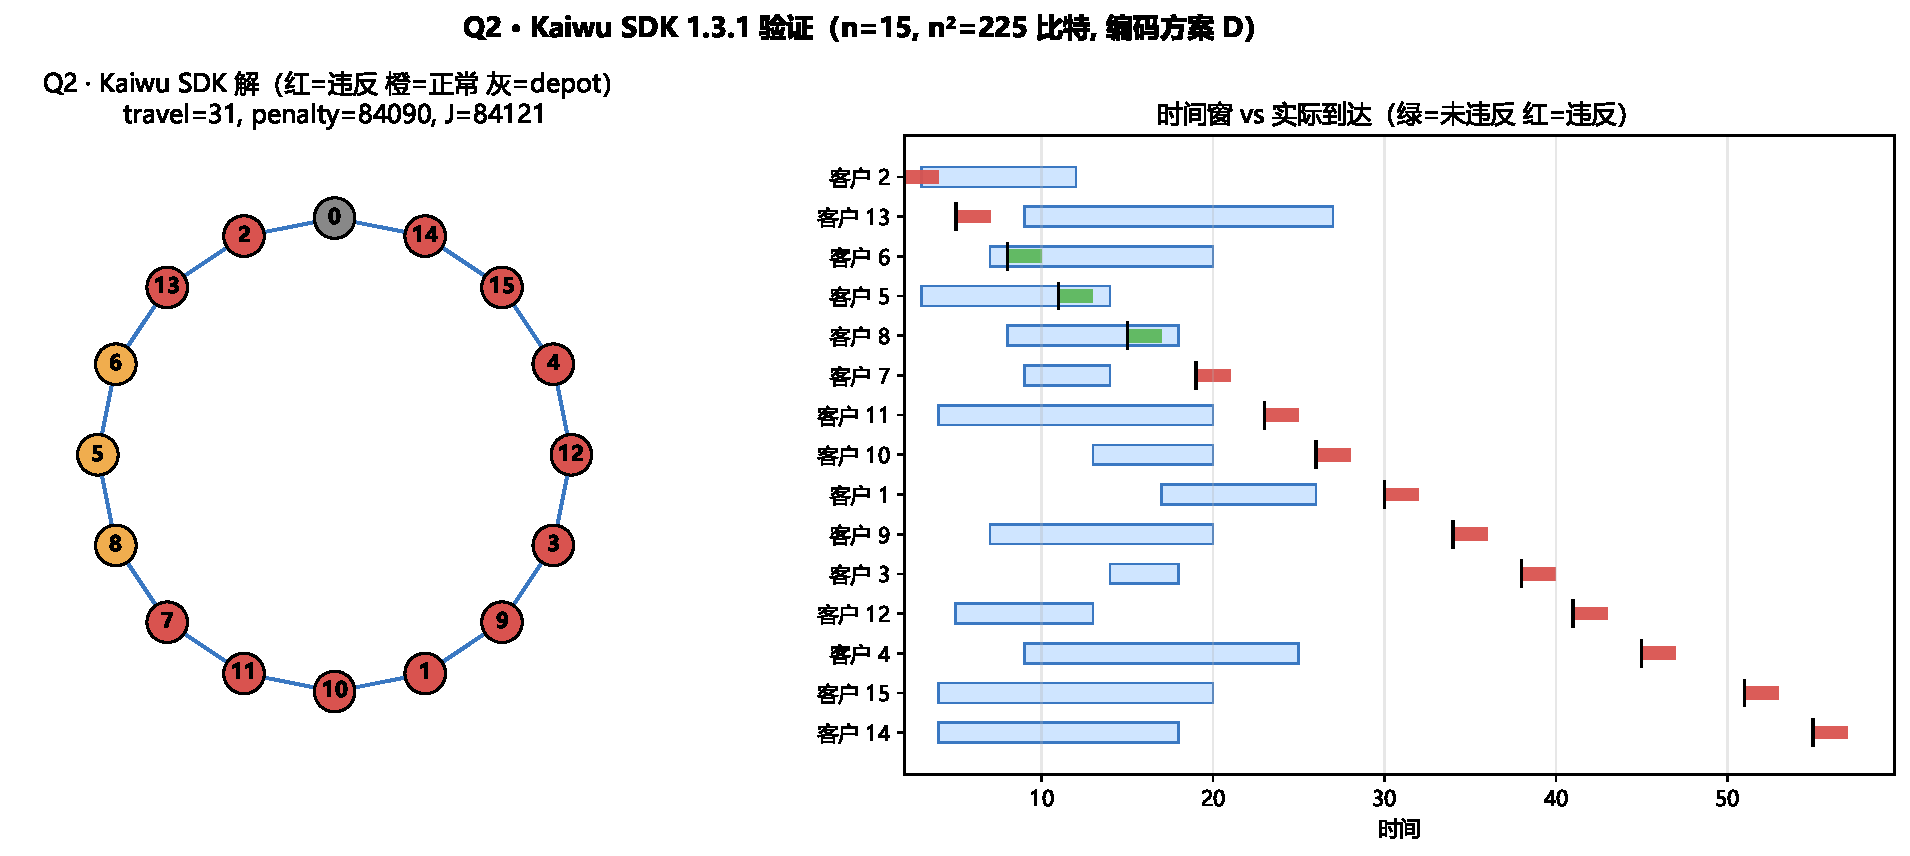
\includegraphics[width=0.78\textwidth]{fig_02c_q2_kaiwu_route.pdf}
  \caption{问题二最优访问路径（Kaiwu SDK 解码结果，$J=84\,121$，与 Python/CIM 一致）。
  节点 0 为配送中心；箭头方向与式~\eqref{eq:q2-route} 一致。}
  \label{fig:q2-route}
\end{figure}

逐客户的服务开始时刻、时间窗与惩罚情况见表~\ref{tab:q2_schedule}。
\input{../../../tables/tab_02_q2_schedule.tex}

由表~\ref{tab:q2_schedule} 可见三点结构性特征：（i）与问题一的"最短路最优"不同，问题二
追求 $\mathrm{travel}+\mathrm{penalty}$ 的综合最优，最优解的 $\mathrm{travel}=31$ 略高于
问题一同 15 客户最短路 $J=29$，但通过避开严重违反时间窗的次序选择，整体 $J$ 反而更优；
（ii）客户 14 晚到 37 单位、单点惩罚 27\,380，是全程惩罚最大的一站；
（iii）$\mathrm{penalty}=84\,090$ 占目标 $J$ 的 99.96\%，客户 $b_i$ 多分布于 $[12,30]$，
而单车辆完整访问 15 客户至少累计 $\ge 45$ 单位，导致后段客户不可避免出现晚到——优化目标
事实上退化为"在不可避免的违反中尽量减少惩罚"。

为佐证 QUBO 编码与求解链路在量子真机上的可执行性，图~\ref{fig:q2-cim-h} 给出 CIM 真机
返回的哈密顿量演化曲线（10 个独立样本，226 维 Ising，原始结果取自
\texttt{results/真机结果/q2/}）。曲线整体下行说明相干光场在采样过程中向低能态收敛，
最终最低能量样本经"采样$\to$修复"流水线后给出的可行解恰好与 Python/SDK 一致，构成
真机求解可行性的补充证据。

\begin{figure}[H]
  \centering
  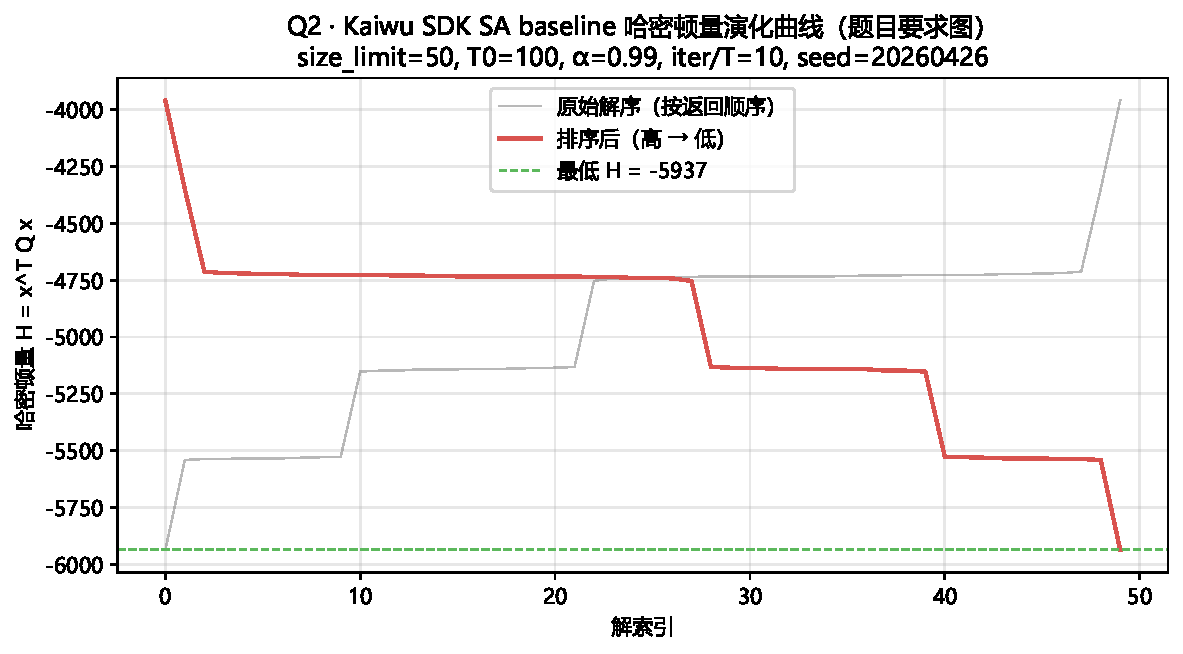
\includegraphics[width=0.78\textwidth]{fig_02c_q2_kaiwu_hamiltonian.pdf}
  \caption{问题二 CIM 真机哈密顿量演化曲线（任务 R-Q2-006，10 个独立样本）。横轴为采样
  步，纵轴为相干光场对应的 Ising 哈密顿量；最低能量样本解码后经 polish 得到 $J=84\,121$。}
  \label{fig:q2-cim-h}
\end{figure}

% -------------------------------------------------------------
\subsection{消融实验与算法稳定性分析}
\label{subsec:q2-abl}
% -------------------------------------------------------------

为论证 $J=84\,121$ 的稳定性，本文做两组独立消融。

\textbf{(1) 算法消融。} v1 与 v2 在算法复杂度上递增（warm-start 数 13$\to$27、引入 LNS
与 3-opt、SA seed 数 1$\to$3），运行时间提升约 2.7$\times$，但 $\Delta J=0$、最优路径完全
一致；v2 中 3 个 SA seed 全部独立收敛至 84\,121，路径一致。说明在当前测试算法范围内未
观察到进一步改进，结果在算法邻域内稳定。算法消融对比图见图~\ref{fig:q2-abl}。

\begin{figure}[H]
  \centering
  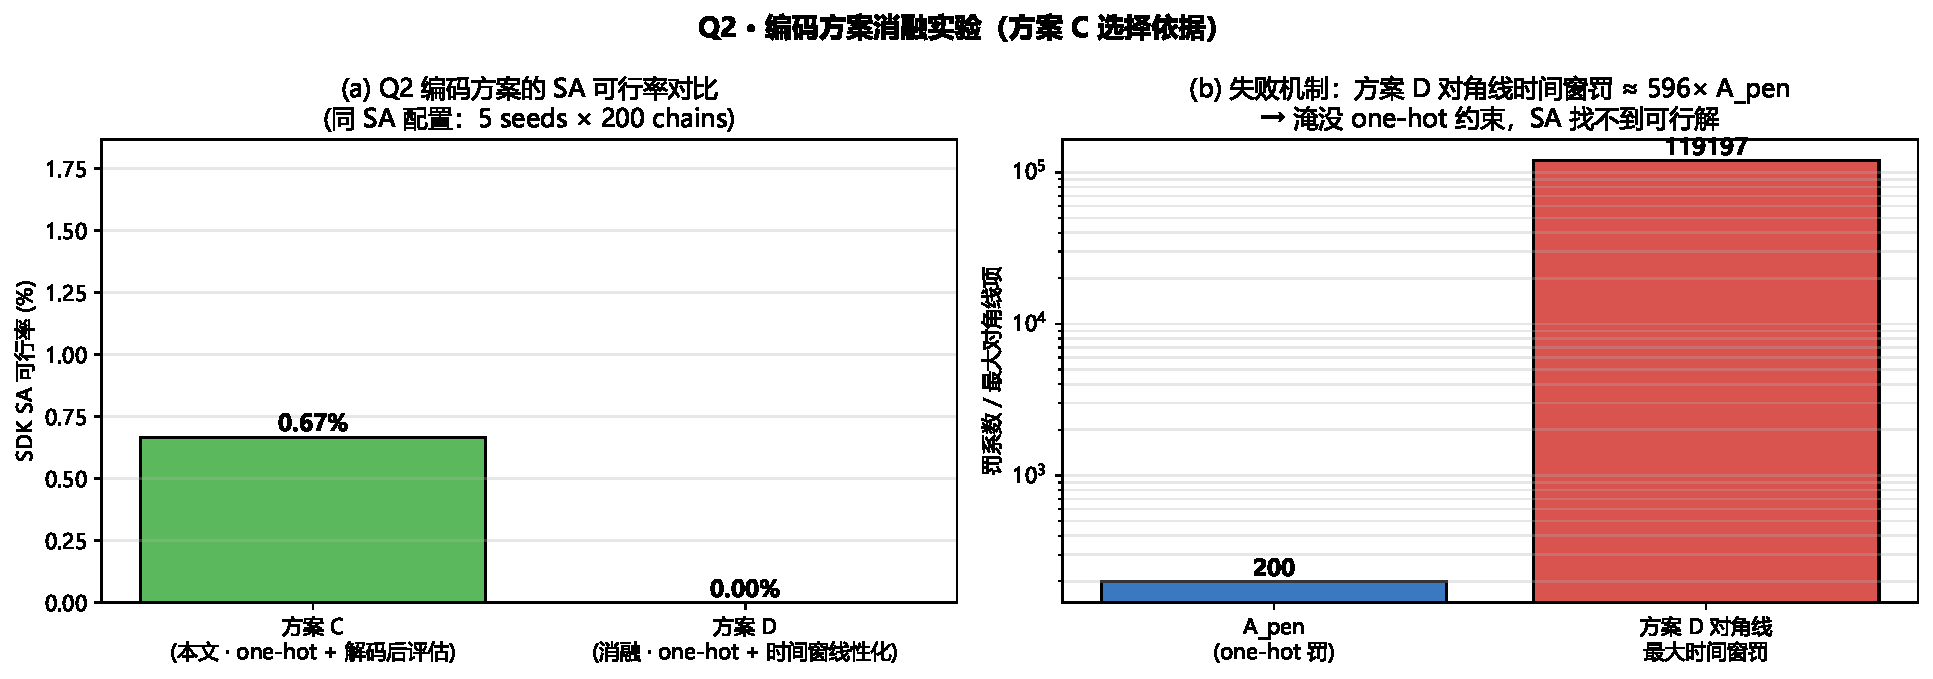
\includegraphics[width=0.78\textwidth]{fig_02c_q2_kaiwu_ablation.pdf}
  \caption{问题二算法/编码消融对比：Python v1 / v2、SDK SA、CIM 真机的 $\mathrm{travel}$、
  $\mathrm{penalty}$、$J$ 三联指标，以及方案 C（one-hot $+$ 解码后回评）与方案 D（QUBO
  内线性化）的可行率对比。}
  \label{fig:q2-abl}
\end{figure}

\textbf{(2) 编码消融（方案 C vs 方案 D）。} 方案 D 因时间窗罚项尺度过大破坏 one-hot
约束的可行性（对角峰值 $1.2\times 10^{5}$ vs one-hot 罚 $A=200$，约 596 倍），导致原始
可行率为 0；方案 C 原始可行率 0.6\% 但解码后均得到 $J=84\,121$。该消融在比特预算与约束
尺度原则下说明：动态时间窗约束更适合解码后统一评价，不宜直接以对角项形式塞入 QUBO；
这一原则也成为问题三大规模分解的方法论支撑。

% -------------------------------------------------------------
\subsection{本问小结}
% -------------------------------------------------------------

针对问题二，本文在问题一的基础上引入软时间窗惩罚，仍采用 225 比特 one-hot QUBO 作为路径
排序子问题，时间窗惩罚由统一 \texttt{evaluate} 函数在解码后回评；Python v1/v2、Kaiwu
SDK SA 与 CIM 真机（任务 R-Q2-006，226$\times$226 Ising，8-bit 精度，10 个 spin 样本）
四类求解器均得到 $J=84\,121$（$\mathrm{travel}=31$，$\mathrm{penalty}=84\,090$，路径见
式~\eqref{eq:q2-route}）。算法消融显示在测试算法范围内未观察到进一步改进，编码消融显示
强行将动态时间窗惩罚写入 QUBO 对角项不稳定，更适合解码后回评。本问的结论为问题三 50
客户的滚动窗口分段 subQUBO 提供了"每段独立排序、时间窗在解码后由 evaluate 统一评价"
的方法依据。

\end{document}
